\chapter{Graphrepräsentationen}
\label{chap:graph_data}

Das nachfolgende Kapitel basiert, sofern nicht anders vermerkt, auf~\cite{linkeddatatools}.

Eine der Grundlagen der semantischen Daten, sowie speziell von semantischen Netzen, bilden Graphen. Man spricht in diesem Zusammenhang auch von Graphdatenbanken.

Der Unterschied gegenüber den anonsten gängigen Datenbanken, wie den relationalen oder hierarchischen Datenbanken, liegt vorallem darin, dass die Objekte beliebig verknüpft sein können.

Eine Graphdatenbank ist analog einem Graphen aufgebaut. Sie nutzt also dessen Struktur, bestehend aus Knoten, Kanten und Eigenschaften, um Daten bzw. Wissen darzustellen und abzulegen. Eine Graphdatenbank ist also ein Graph mit zyklenfreier Nachbarschaft. Dies bedeudet, dass jedes Element einen direkten Verweis auf seine benachbarten Elemente enthält und somit keine Abfragen auf dessen Relationen notwendig sind.

Die Knoten einer Graphdatenbank repräsentieren Entitäten, Eigenschaften sind auf Knoten bezogene Informationen. Kanten verbinden Knoten mit Knoten oder Knoten mit Eigenschaften und stellen eine Beziehung zwischen diesen dar.

\begin{figure}[htbp]
\centering \rotatebox{0}{\scalebox{0.5}[0.5]{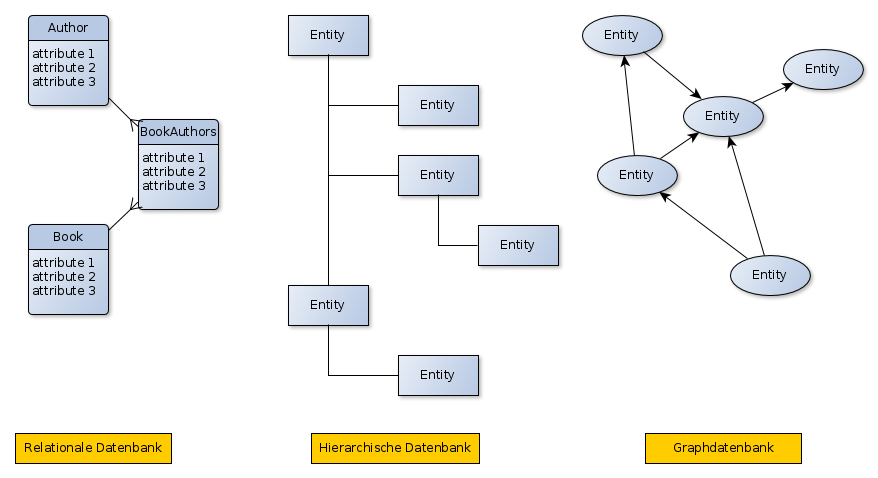
\includegraphics{bilder/datenbanktypen.png}}}
\caption{Darstellung der verschiedenen Datenbanktypen.\label{fig:datenbanktypen}\protect\footnotemark}
\end{figure}
\footnotetext{Eigene Darstellung mittels yEd}

\newpage

Gegeben seien die folgenden Aussagen über Hotels:
\lstset{caption={Aussagen über Hotels\protect\footnotemark},captionpos=b}
\begin{lstlisting}
    Ein Wellnesshotel ist ein Hotel.
    Ein Familienhotel ist ein Hotel.
    Wellnesshotels sind mit Familienhotels verwandt.
\end{lstlisting}

Verwendet man nun diese Aussagen über Hotels um daraus eine Graphdatenbank zu erstellen, so ergibt sich folgende Graphdatenbank:
\begin{figure}[htbp]
\centering \rotatebox{0}{\scalebox{0.5}[0.5]{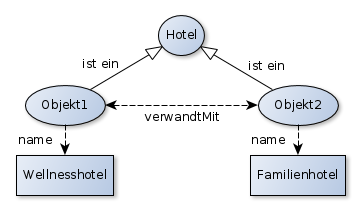
\includegraphics{bilder/hotels_graph.png}}}
\caption{Aussagen über Hotels als Graphdatenbank.\label{fig:hotels_graphdatenbank}\protect\footnotemark}
\end{figure}
\footnotetext{Eigene Darstellung mittels yEd}

In der Graphdatenbank existieren also zwei Objekte, \textit{``Objekt1''} und \textit{``Objekt2''}, mit den Eigenschaften \textit{``ist ein''}, \textit{``verwandtMit''} und \textit{``name''}.

\newpage

\noindent\rule[1ex]{\textwidth}{1pt}
\begin{wrapfigure}[5]{l}{0.1\textwidth}
    \vspace{-12pt}
    
\includegraphics[width=0.1\textwidth]{bilder/elephant.png}
\end{wrapfigure}
\label{elephant_graph_data}
Möchte man nun eine Graphdatenbank als Grundlage für eine semantische Datenbank aufbauen, so empfiehlt es sich, zuerst die wichtigsten Klassen und Individuen  zu identifizieren. Es lohnt sich sicherlich auch, wenn man beim Aufbau schrittweise vorgeht.

Nimmt man das Beispiel des Reispeplaners, macht es sicherlich Sinn, wenn man nicht von Anfang an versucht eine komplette Reise abzubilden, sondern zuerst mit der Abbildung lokaler Ausflüge beginnt. Diese können später mittels Logik zu einer Reise kombiniert werden.

Nach einiger Überlegung ergeben sich die Klassen \textit{Ausflug}, \textit{Land}, \textit{Region} und \textit{Ort}. Doch wie gelangt man zu diesen? Unserer Erfahrung nach lohnt es sich, wenn man konkrete Fragen stellt, welche die semantische Datenbank schlussendlich beantworten können soll. Es ist auch hilfreich, sich praktische Beispiele der Anwendung solch einer Datenbank zu überlegen.

So könnte eine konkrete Anwendung zum Beispiel eine Familie sein, welche einen eintägigen Ausflug planen möchte und deren Kinder bereits in einem Alter sind, in welchem sie Beschäftigung benötigen. Dies führt schlussendlich zu den Kriterien \textit{familienfreundlich}, \textit{regional} und \textit{actionreich}. Dies sind jedoch reine Überlegungen für die spätere Entwicklung. Eine Graphdatenbank in diesem Sinne nicht ohne Weiteres komplexe Anfragen im Sinne der genannten Kriterien beantworten. Man könnte dies statisch modellieren, in dem man den Objekten die Kriterien zuweist, dies würden jedoch den Vorteil einer semantischen Datebank, dass Schlüsse aufgrund von komplexen Zusammenhängen gewonnen werden können, zu Nichte machen.

Hat man die Klassen und die Kriterien identifiziert, fällt auf, dass so noch keine konkreten Anfragen beantwortet werden können. Es fehlen die Individuen und die Relationen. Es wird daher ein Individuum für einen Ausflug, \textit{Seilpark Balmberg}, erstellt. Nun erscheint es logisch, dass ein Land in Regionen unterteilt ist und diese wiederum Orte beinhalten. Dies kann über die Relationen \textit{hatRegion} und \textit{hatOrt} abgebildet werden.

\begin{figure}[H]
\centering \rotatebox{0}{\scalebox{0.5}[0.5]{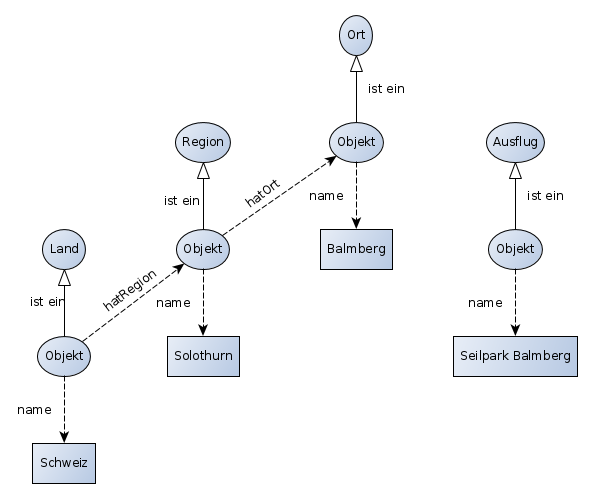
\includegraphics{bilder/graphen_beispiel_1.png}}}
\caption{Beispiel einer Graphdatenbank basierend auf dem Beispiel eines Reiseplaners\label{fig:protegebeispiel}\protect\footnotemark}
\end{figure}
\footnotetext{Eigene Darstellung mittels yEd\footnote{\url{http://www.yworks.com/en/products/yfiles/yed/}}}

Wie in der Grafik ersichtlich ist, hat jedoch das Individuum \textit{Seilpark Balmberg} momentan keine Relation/en zu anderen Individuuen. Zum jetzigen Zeitpunkt ist nicht klar, wie dieses so verknüpft werden kann, dass ein Mehrwert mi Sinn von Abfragemöglichkeiten generiert wird.

\vspace{0.1pt}
\noindent\rule[1ex]{\textwidth}{1pt}

Da eine Graphdatenbank eher eine hohe Abstraktionsebene darstellt, werden Wissensrepräsentationsformen sowie die Anwendung dieser im folgenden Kapitel ---~\ref{chap:wissensrepFormen}~\nameref{chap:wissensrepFormen}--- genauer erläutert.
